

\section{Fermi surface nesting as a pairing mechanism}

The charge carrier in a superconducting condensate is a Cooper pair - a quasi-particle comprising of a bound state of two electrons or two holes with opposite spin and momentum. Evidence for this configuration arises as a natural result of the Ginzberg-Landau model which, when applied to a superconducting system, gives the charge of the quasi-particle carriers as $2e$, where $e$ is the charge of an electron. Given that due to their like charges two free electrons repel, it is natural to ask what could overcome the electromagnetic force to cause these electrons to remain bound in this quasi-particle state.

Bardeen, Cooper and Schreiffer established much of the theoretical basis --- from which the Ginzberg--Landau model can be derived --- in \textit{BCS theory} (named after the authors) and within the framework of BCS theory, wrote a 1957 paper\cite{Bardeen1957} detailed a pairing mechanism known as the \textit{BCS model} which would explain how these electron remained bound together. The model is based around the concept of phonons scattering off ions which well suited the superconducting materials known at the time. Phenomenologically, the mechanism of attraction is straightforward. Electrons moving through a crystal lattice attract ions on the lattice sites. These heavy ions respond slowly and are drawn in \textit{behind} the electron. This has the effect of both screening the negative electron charge as well as providing an attractive positive potential for any electron following the original electron. The net effect is the leading electron draws the following electron in its wake, thus coupling them with one another. The wavelike distortion of the ions in the lattice can be considered as a phonon, and the interaction between the electrons and the lattice can be modelled as electron--phonon--electron scattering.

The BCS model on top of BCS theory accurately describes what we now know as \textit{conventional superconductivity}, that is pairing which forms a spin-singlet state ($S=0$) and which has zero orbital angular momentum ($L=0$). It was not until the discovery of superfluidity\footnote{Superfluidity and superconductivity share much of the same physics although rather than electrons or holes pairing, molecules pair instead. Parallels betwen the two are discussed in ref.\cite{Annett2010}} in $^3$He in 1972\cite{Osheroff1972} that it became apparent that there may exist forms of pairing that resulted in spin-triplet pairing state ($S=1$) with $L>0$. This was later confirmed when superconducting analogues were found in the form of heavy Fermion materials. What really spurred the explosion in interest though was the 1986 discovery by Bednorz and M\"uller\cite{Bednorz} of high transition temperature (\Tc) superconductivity in the cuprates and, more recently, the `pnictides' by Kamihara et al.\cite{Kamihara2008}. The cuprate class of materials that Bednorz and M\"uller found to be superconducting have \Tc~s far in excess of any previously known superconducting materials and although the BCS model phonon pairing may play a part, the predominant pairing mechanism in the \highTc materials is likely to be something else entirely.

\subsection{The case against conventional superconductivity in \highTc}

There is a great deal of evidence in the literature for non-BCS model pairing in the \highTc and heavy Fermion materials. Although the pairing wavefunction cannot be measured directly with current techniques, experiments indirectly infer \textit{unconventional} i.e. non s-wave, BCS-model, characteristics. For example, analysis on penetration depth measurements of YBa$_2$Cu$_3$O$_{7-\delta}$ show power law behaviour\cite{Annett1991}, indicating that there exists states within the momentum averaged gap. SQUID measurements and Josephson tunneling experiments on the same material have confirmed alternating phase of the condensate wavefunction which points strongly to \DxTwoyTwo--wave symmetry\cite{VanHarlingen1994} (see also refs. therein). As for other cuprate materials, specific heat measurements on \BSCO\cite{Wang2011}, as well as peentration depth measurements on LSCO\cite{Froehlich1996} have also proved consistant with $d$-wave pairing. 

More evidence against conventional superconductivity include the unusual normal state (i.e. non-superconducting) state properties of the cuprates and heavy Fermion materials. The BCS model is grounded in Landau Fermi liquid theory which models interacting itinerent electrons with quasiparticles of heavier effective mass than ordinary electrons and holes. A hallmark of Fermi liquid behaviour is a $T^2$ dependence of the resistance, however experiments on the cuprate La$_{2-x}$Sr$_{x}$CuO$_4$\cite{Cooper2009} and a heavy Fermion material\cite{Custers2003} have demonstrated fractional power law behaviour, $T^\gamma$ where $1 < \gamma < 2$, at temepratures above the superconducting transition. Given that the Fermi liquid model breaks down in these examples, it follows that the BCS-model also is likely on shaky ground for these materials.

There are several arguments against phonons as the sole pairing mechanism in the pnictide case, Boeri et al.\cite{Boeri2008} and Mazin et al.\cite{Mazin2008} present calculations showing that the magnitude of the phonon pairing strength is not adequate for the high \Tc values attained in LaAsOF, Haule et al.\cite{Haule2008} note in the same material that the gradient of the density of states (DOS) at the Fermi level is such that you would expect an increase in DOS and hence \Tc with hole doping if the BCS model held, however the reverse is true. Non Fermi-liquid behaviour was demonstrated in the \BaFePAs series\cite{Jiang2009,Kasahara2010} and evidence for nodes in the gap function have been found in LaFePO\cite{Fletcher2009} and the \BaFePAs series\cite{Zhang2011,Yamashita2011a,Suzuki2011} although not in \TODO{Finish this}

It is interesting to note that Unlike the cuprates which universally show a \DxTwoyTwo gap symmetry, the pnictide materials are note all alike. As a result, it may prove that the nature of the supercondcutivity may not be universal amongst the pnictide materials. Irrespective of this, there is no evidence for BCS model pairing in the pnictide materials and in many cases, BCS pairing has been shown to be insufficient.


\subsection{Spin-fluctuations}

Soon after the discovery of the pnictide materials, a possible pairing mechanism was proposed based on spin density wave fluctuations. The original paper suggested a $s_{\pm}$ gap symmetry which does not feature any nodes however 

\subsection{Pnictides}

Some arguments against the BCS theory of pairing \cite{Haule2008,Yndurain2009,Mazin2008} based on arguments of 

FS nesting not the only cause of spin-fluctuations, also can be caused by frustrated superexchange for example \TODO{Finish this}

Spin fluctuations mediate a repulsive interaction between Cooper pair candidates.

The anisotropic BCS equations specify that repulsive coupling between carriers can be pairing provided the order parameter changes sign over the coupling vector.


There are several proposed mechanisms presently on offer including charge fluctuations resulting in large ion polarisation \cite{Berciu2009}, however this was contested by Mazin and Schmalian\cite{Mazin2009}.


Of these theories, the one with arguably the most traction at present is that of spin-fluctuation mediated pairing. 

\TODO{What actually is the cause of the attraction in the nesting picture? ... Spin fluctuation intereaction in real space is approximately propoprtional to the dipole interaction $V=-\mu . \mu \chi(r)$}%\cite{Bergemann2003}

Strong correlations - the interaction energy is much greater than the kinetic energy for the states
When correlations present, Cooper pairs are assumed to be pairs of Landau quasiparticles


% The Stoner condition of $\mathcal{N}_0 I > 1$ -- where $\mathcal{N}_0$ is the density of states at the Fermi energy and $I$ is the molecular field constant, that scales the magnetism given a field -- indicates an energy instability\cite{Kubler2000}

\subsection{The \BaFePAs series}

In order to explore the role of nesting in the \highTc superconductors, an investigation at Bristol was undertaken on the Fermiology of the \BaFePAs series by studying angle resolved \ac{dHvA} oscillations and in particular the end-member, \BaFeP.

The \BaFePAs series is one of many that stem from the parent compount \BaFeAs, although unlike the electron doped \BaCoFeAs and the hole doped \BaKFeAs series, the \BaFePAs progression is entirely isovalent meaning that the changes affected due to the P substitution are due to structure and chemical pressure rather than additional charge carriers. Nonetheless, superconductivity occurs with a very similar phase diagram as with the charge-doped examples in the same `$122$' family of iron-pnictide materials.\footnote{See for example figure~1 in ref.\cite{Paglione2010}}. 

At $x=0$ the \BaFePAs series begins at \BaFeAs, a compound which becomes antiferromagnetic at around \unit{138}{\kelvin}, and moves with increasing $x$ towards \BaFeP which is metallic to low temperatures. Neither end members are superconducting, however as As is substituted for P, the low temperature antiferromagnetic state decays, giving way to superconductivity which kicks in at approximately $x=0.18$ and increases to the optimal substitution of $x=0.31$. Superconductivity then decreases until it gives way to a paramagnetic ground state at around $x=0.71$. Figure~\ref{Fig:Intro:PhaseDiagram} shows the phase diagram adapated from ref. \cite{Nakai2010a} as determined by resistivity measurements. 
\begin{figure}[htbp]
    \begin{center}
        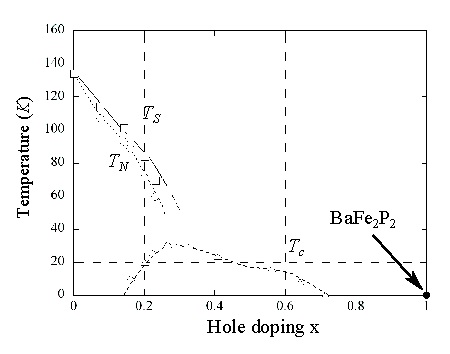
\includegraphics[scale=1.0]{Chapter-Introduction/Figures/PhaseDiagram/PhaseDiagram}
        \caption{Phase diagram adapted from ref \cite{Nakai2010a} measured by resistivity. $T_s$, $T_N$ and $T_c$ are the structural transition, the antiferromagnetic transition and the superconducting transition temperatures respectively.}
        \label{Fig:Intro:PhaseDiagram}
    \end{center}
\end{figure}
Also detailed in the phase diagram is the structural transition which occurs as the tetragonal $I4/mmm$ cell moves to an orthorhombic cell as it passes below the line marked $T_s$. This is a feature which is common to many of the `$122$' pnictide materials.

 The progression along the series is isovalent since P and As are in the same periodic group -- group $V$. The net effect of the substitution is to apply an increasing chemical pressure as $x$ moves towards $1$. Several reports show that applying high \textit{physical} pressure ($\sim$\unit{5}{\giga\pascal}) to \BaFeAs results in a similar phase diagram with an antiferromagnetic phase and superconductivity up to $\sim$\unit{30}{\kelvin}~\cite{Yamazaki2010,Colombier2009,Alireza2009} with Klintberg \textit{et al.}\cite{Klintberg2010} presenting a direct comparison between the two types of pressure. As pressure is applied, the unit cell $a$ axis shrinks slightly less than the $c$ axis ($\sim3\%$ c.f. $\sim4.5\%$ respectively). Interestingly the $c$ axis shrinking largely occurs in the Fe-Pnictide plane leading to some theories of the superconductivity emerging from the tetrahedral bond angle between the Fe and the pnictigen. \TODO{ref read Kuroki}
\begin{figure}[htbp]
    \begin{center}
        \includegraphics[scale=1.0]{Chapter-Introduction/Figures/UnitCell/UnitCell}
        \caption{The tetragonal unit cell of the 122 \BaFePAs series.}
        \label{Fig:Intro:UnitCell}
    \end{center}
\end{figure}


The \BaFePAs series from a substitution of $x=0.41$--$1.0$ has been previously measured by members of the group at Bristol using dHvA oscillations\cite{Shishido2010}. As suggested in the Shishido reference, since dHvA has been observed across such a large range of substitutions, it implies that the material is not prone to disorder as is the case in many charge doped series \TODO{Need ref} making the series an excellant candidate for dHvA studies. This could be explained by the fact that the substitution is isovalent and that there is relatively little contribution at the Fermi surface from the pnictide sites\footnote{See for example, the orbital character for the iron sites from \ac{DFT} calculations presented later in this chapter} where the substitution takes place, meaning the Fermi surface should not be strongly disrupted when traversing the series. The Fermi surfaces from the Shishido paper have been characterised for x ranging from $0.41$ to $1$ for electron sheets only but have clearly shown that the DFT calculations consistently overestimate the size of the surfaces. They also show a linear progression of the electron orbit sizes which is proportional to $x$. Moreover, dHvA measurements on the material with $x=0.63$ have been performed where one of the hole surface extrema was observed\cite{Analytis2010c} however DFT calculations as well as comparisons with \SrFeP\cite{Analytis2009} give evidence for a second hole Fermi surface for materials towards the P end of the series, (towards the As end of the series, there appears this second hole and a \textit{third} hole surface similar but smaller to the other hole sheets). If the electron Fermi surfaces are oversized in the DFT calculations, then the hole Fermi surface volumes should also be oversized in order to remain compensated (electrically neutral). What is not clear though is whether the \textit{shapes} of the hole pockets are also altered in the compounds leading to \BaFeP. DFT calculations show the larger of the hole pockets in particular undergoing significant geometric changes, specifically in that it becomes much more three dimensional as P substitution becomes more complete. The Fermi surface of the opposite end-member, \BaFeAs, has been fully characterised by previous ARPES measurements\cite{Kondo2010a} and dHvA\cite{Terashima2011, Analytis2010b}. Coupled with a full characterisation of the fermiology of \BaFeP, this data can be used to interpolate Fermiology of the hole pockets between end members thus completing the partial determination of the Fermi surfaces of the intermediary compounds.

The ARPES measurements of the Fermi surface of \BaFeAs below the N\'eel temperature concluded that despite some $k_z$ dispersion in the Fermi surfaces, there is adequate nesting to form the antiferromagnetic state. Ab-initio DFT calculations\cite{Shishido2010} of the paramagnetic state have shown the $k_z$ dispersion increasing with increasing P, with the outer hole pockets becoming more three-dimensional through the progression providing the partial nesting conditions necessary for pair forming SDW fluctuations described in section\ref{Sec:1:Nesting}. One caveat is that these calculations do not take into account the structural changes below $T_s$, another caveat is that they do not consider Fermi surface reconstruction due to the observed commensurate antiferromagnetic order. To fully settle the issue of the nature of the nesting in the superconducting state, experimental determination of the Fermi surfaces of the series is necessary, a good guide to which can be obtained from study of the end-members.


This thesis presents data which details the full Fermi surface of \BaFeP including an elucidation of the shape of the 3D outer hole surface. Partial nesting is detailed between the outer hole surface and the inner electron surface with $q=(\pi, \pi, \pi/2)$ meaning the phenomenum persists through to the end member of the series. Also presented are effective mass measurements which show relatively small mass enhancements implying weak carrier correlations.
